\documentclass[12pt,compress,aspectratio=169]{beamer}
\usetheme{metropolis}
\setbeamersize{text margin left=.5cm,text margin right=.5cm}
\usepackage[lf]{carlito}
\usepackage{siunitx}
\usepackage{tikz}
\usepackage{mathpazo}
\usepackage{bm}
\usepackage{mathtools}
\usepackage[ISO]{diffcoeff}
\diffdef{}{ op-symbol=\mathsf{d} }
\usepackage{xcolor,colortbl}

\setmonofont{Ubuntu Mono}
\setlength{\parskip}{0pt}
\renewcommand{\baselinestretch}{1}

\sisetup{
  inter-unit-product=\cdot,
  per-mode=symbol
}

\tikzset{
  >=latex
}

%\newcommand{\iii}{\hat{\bm\imath}}
%\newcommand{\jjj}{\hat{\bm\jmath}}
%\newcommand{\kkk}{\hat{\bm k}}


\usetikzlibrary{decorations.pathmorphing,patterns}

\title{Class 12: Orbital Mechanics}
\subtitle{Advanced Placement Physics C}
\author[TML]{Dr.\ Timothy Leung}
\institute{Olympiads School}
\date{Updated: Summer 2022}

\newcommand{\pic}[2]{
  \includegraphics[width=#1\textwidth]{#2}
}
\newcommand{\eq}[2]{
  \vspace{#1}{\Large
    \begin{displaymath}
      #2
    \end{displaymath}
  }
}
%\newcommand{\iii}{\ensuremath\hat{\bm{\imath}}}
%\newcommand{\jjj}{\ensuremath\hat{\bm{\jmath}}}
%\newcommand{\kkk}{\ensuremath\hat{\bm{k}}}
\newcommand{\iii}{\ensuremath\hat\imath}
\newcommand{\jjj}{\ensuremath\hat\jmath}
\newcommand{\kkk}{\ensuremath\hat k}



\begin{document}

\begin{frame}
  \maketitle
\end{frame}


\section{Orbits}

\subsection{Orbital Velocity and Escape Velocity}

\begin{frame}{Newton's Thought Experiment}
  In \emph{Treatise of the System of the World}, the third book in
  \emph{Principia}, Newton presented this thought experiment:
  \begin{center}
    \pic{.8}{figure-5}
  \end{center}
  \begin{itemize}
  \item How fast does the cannonball have to travel before it goes around Earth
    without falling? (i.e.\ goes into orbit)
  \item How fast does the cannonball have to travel before it never comes back?
  \end{itemize}
\end{frame}



\begin{frame}{Relating Gravitational and Centripetal Force}
  Assuming a small mass $m$ in circular orbit around a much larger mass $M$.
  The required centripetal force is supplied by the gravitational force:
  
  \eq{-.1in}{
    F_g=F_c\quad\longrightarrow\quad \frac{GMm}{r^2}=\frac{mv^2}r
  }

  \vspace{-.1in}Solving for $v$, we obtain the \textbf{orbital velocity}
  $v_\text{orbit}$, which does not depend on the mass of the small object in
  orbit:

  \eq{-.1in}{
    \boxed{v_\text{orbit}=\sqrt{\frac{GM}r}}
  }

  This equation is only applicable for perfectly circular orbits.
\end{frame}



\subsection{Escape Velocity}

\begin{frame}{Escape Velocity}
  An object can leave the surface of Earth at any speed. But when all the
  kinetic energy of that object is converted to gravitational potential energy,
  it will return back to the surface of the earth. There is, however, a
  \emph{minimum} velocity at which the object \emph{would not} fall back to
  Earth.
\end{frame}



\begin{frame}{Escape Velocity}
  The calculation for escape is a simple exercise in conservation of energy,
  since gravity is a conservative force, i.e.:

  \eq{-.1in}{
    K + U_g = K' + U_g'
  }
  \begin{itemize}
  \item Initial gravitational potential energy at the surface is:

    \eq{-.1in}{
      U_g=-\frac{GMm}{r_i}
    }
  \item The final gravitational potential energy is at the other side of the
    universe ($r_f=\infty$), where $U_g'=0$. At this point, the object has
    \emph{escaped} the gravitational pull of the planet/star
  \item The minimum kinetic energy at $r=\infty$ is $K'=0$
%  \item The work against gravity converts kinetic energy into gravitational
%    potential energy.
%  \item If you start with \emph{more} kinetic energy than required to do all
%    the work, then the object has
%    planet.
  \end{itemize}
\end{frame}



\begin{frame}{Escape Velocity from Circular Orbits}
  Setting $K$ to equal to $-U_g$:

  \eq{-.1in}{
    \frac12mv_i^2=\frac{GMm}{r_i}
  }

  We can then solve for the initial speed $v_i=v_\text{esc}$
  (\textbf{escape speed} or \textbf{escape velocity}):

  \eq{-.1in}{
    \boxed{v_\text{esc}=\sqrt{\frac{2GM}{r_i}}}
  }

  where $r_i$ is the initial distance from the center of the planet/star. There
  is a simple relationship between orbital speed and escape speed:

  \eq{-.1in}{
    v_\text{esc}=\sqrt2v_\text{orbit}
  }
\end{frame}



\begin{frame}{Example Problem}
  \textbf{Example:} Determine the escape velocity and energy for a
  \SI{1.60e4}{\kilo\gram} rocket leaving the surface of Earth.

  \uncover<2>{
    \vspace{.5in}Note: The equation for the escape speed is based on the object
    have a \emph{constant} mass, which is \emph{not} the case for a rocket
    going into space.
  }
\end{frame}



\begin{frame}{What if I'm not escaping from the surface?}
  Both objects have the same escape velocity:
  \begin{center}
    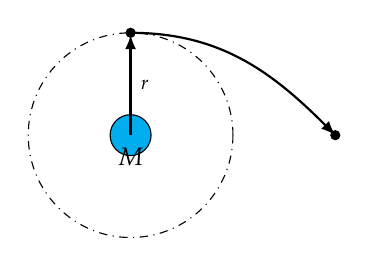
\begin{tikzpicture}[scale=1.3]
      \draw[fill=cyan] circle(.2) node[midway,below]{\scriptsize $M$};
      \draw[dash dot] circle(1);
      \fill (0,1) circle(.05);
      \draw[->,thick](0,0)--(0,.98) node[midway,right]{\scriptsize $r$};
      \fill (2,0) circle(.05);
      \draw[->,thick](0,1) to[out=0,in=135](2,0);
    \end{tikzpicture}
    \hspace{.3in}
    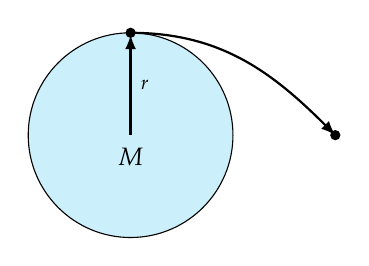
\begin{tikzpicture}[scale=1.3]
      \draw[fill=cyan!20] circle(1) node[midway,below]{\scriptsize $M$};
      \fill (0,1) circle(.05);
      \draw[->,thick](0,0)--(0,.98) node[midway,right]{\scriptsize $r$};
      \fill (2,0) circle(.05);
      \draw[->,thick](0,1) to[out=0,in=135](2,0);
    \end{tikzpicture}
  \end{center}
  The difference is that the object in orbit (left) already has orbital speed
  $v_\text{orbit}$, so escaping from that orbit requires only an additional
  speed of
  
  \eq{-.1in}{
    \Delta v=v_\text{esc}-v_\text{orbit}=(\sqrt2-1)v_\text{orbit}
  }
  \begin{itemize}
  \item What if $v_\text{orbit}<v<v_\text{esc}$?
  \item What if $v<v_\text{orbit}$?
  \end{itemize}
\end{frame}



\begin{frame}{Non-Circular Orbits}
  \centering
  \pic{.6}{newton-cannon-orbital-types-Seeds}
\end{frame}



\subsection{Orbital Energies}

\begin{frame}{Orbital Energies}
  We can obtain the \textbf{orbital kinetic energy} in a perfectly circular
  orbit by using the orbital speed in our expression of kinetic energy:

  \eq{-.1in}{
    K_\text{orbit}=\frac12mv_\text{orbit}^2=\frac12m
    \left(\sqrt{\frac{GM}r}\right)^2=\boxed{\frac{GMm}{2r}}
  }

  We already have an expression for gravitational potential energy:

  \eq{-.1in}{
    U_g=-\frac{GMm}r=-2K_\text{orbit}
  }
  
  The \textbf{total orbital energy} is the sum of $K$ and $U_g$:

  \eq{-.1in}{
    E_T=K_\text{orbit}+U_g=-\frac{GMm}{2r}=-K_\text{orbit}
  }
\end{frame}



\section{Orbital Mechanics}

\begin{frame}{Orbital Mechanics}
  We turn our attention to applying the law of universal gravitation to the
  orbital motion of planets and stars in our solar system.
\end{frame}



\begin{frame}{Properties of Gravitational Force}
  Two properties of gravity are crucial to understanding of orbital mechanics:
  \begin{enumerate}
  \item Gravity is a \emph{conservative force}, in that
    \begin{itemize}
    \item The total mechanical energy of objects under gravity is constant
    \item Work done by gravity converts gravitational potential energy $U_g$
      into kinetic energy $K$; work against gravity converts $K$ into $U_g$
    \end{itemize}
  \item Gravity is a \emph{central force}, in that
    \begin{itemize}
    \item Gravitational force $\vec F_g$ is always in the $-\hat r$ direction,
      i.e.\ $\vec F\times\vec r=\vec 0$
    \item Therefore gravity doesn't generate any torque
    \item And therefore angular momentum $\vec L$ is constant
    \end{itemize}
  \end{enumerate}
  These two properties are true regardless of the shape of the orbit, and even
  for objects that are not in orbit at all!
\end{frame}


\begin{frame}{Kepler's Laws of Planetary Motion}
  Johannes Kepler (1571--1630) formulated the \textbf{laws of planetary motion}
  between 1609 to 1619, by interpreting planetary motion data from his teacher,
  Tycho Brahe. It is an improvement over the heliocentric theory of Nicolaus
  Copernicus. Expressed in modern language:
  \begin{enumerate}
  \item\textbf{Law of ellipses:} The orbit of a planet is an ellipse with the
    Sun at one of the two foci.
  \item\textbf{Law of equal areas:} A line segment joining a planet and the Sun
    sweeps out equal areas during equal intervals of time
  \item \textbf{Law of periods:} The square of the orbital period of a planet
    is proportional to the cube of the semi-major axis of its orbit.
  \end{enumerate}
  (For anyone who is interested, there is a handout with the proofs of Kepler's
  laws using Newton's laws of motion.)
\end{frame}



\subsection{Second Law}

\begin{frame}{Kepler's Second Law: Law of Equal Areas}
  \begin{center}
    \fbox{
      \begin{minipage}{.97\textwidth}
        \textbf{Law of Equal Areas: A line segment joining a planet and the Sun
          sweeps out equal areas during equal intervals of time}
      \end{minipage}
    }

    \pic{.4}{201532-132212364-3243-planet}
  \end{center}
  The second law of planetary motion is the easiest to proof, by applying the
  conservation of angular momentum $\vec L=m(\vec r\times\vec v)$ (gravity is a
  central force).
\end{frame}


%\begin{frame}{Kepler's Second Law: Law of Equal Areas}
%  \begin{center}
%    \fbox{
%      \begin{minipage}{.9\textwidth}
%        \textbf{A line segment joining a planet and the Sun sweeps out equal
%          areas during equal intervals of time}
%      \end{minipage}
%    }
%  \end{center}
%  \begin{columns}
%    \column{.3\textwidth}
%    \begin{tikzpicture}[scale=1.3]
%      \fill[gray!45](0,0)--(2,3)--(3,2.8)--cycle;
%      \node at (1.7,2) {$d\vec{A}$};
%      \draw[->,thick](0,0)--(2,3)
%      node[midway,left]{$\vec r$} node[pos=.95,right]{$\alpha$};
%      \draw[->,thick](2,3)--(3,2.8) node[midway,above]{$d\vec r$};
%      \draw[dashed](3,2.8)--(0,0);
%      \fill[black](0,0) circle(.07) node[right]{\tiny\text{Sun}};
%      \fill[black](2,3) circle(.035)node[above]{\tiny\text{Planet}};
%    \end{tikzpicture}
%    \column{.7\textwidth}
%    The infinitesimal area $d\vec{A}$ swept out by an object (such as a planet)
%    as it moves in orbit by an infinitesimal amount $d\vec r$ is given by:
%    
%    \eq{-.4in}{
%      dA=\frac{1}{2}rdr\sin\alpha
%      \;\rightarrow\;
%      d\vec{A}=\frac{1}{2}\vec r\times d\vec r
%    }
%
%    \vspace{-.15in}Its time derivative is called the \textbf{areal velocity}:
%      
%    \eq{-.15in}{
%      \frac{d\vec{A}}{dt}
%      =\frac{1}{2}\vec r\times\frac{d\vec r}{dt}
%      =\frac{1}{2}\vec r\times\vec{v}
%    }
%  \end{columns}
%\end{frame}



\begin{frame}{Kepler's Second Law: Law of Equal Areas}
  The rate of change of the area ($\dl A/\dl t$) swept out by a planet (called
  the \textbf{areal velocity}) is given by:

  \eq{-.1in}{
    \diff At=\frac L{2m}=\text{constant}
  }

  The rate a planet sweeps out the area in orbit is its angular momentum around
  the sun divided by twice its mass.
\end{frame}



\subsection{First Law}

\begin{frame}{Kepler's First Law: Law of Ellipses}
  Proofing Kepler's first law requires some understanding the ellipse. If
  the law is true, then orbital motion must agree with the equations of an
  ellipse.
  \begin{columns}
    \column{.3\textwidth}
    \centering
    \pic{1.1}{elliporb}

    \column{.7\textwidth}
    \begin{itemize}
    \item $r' + r =2a$
    \item The area of the ellipse is $A=\pi ab$
    \item The relationship between $r$ and $\theta$ given by:

      \eq{-.1in}{
        r=\frac{a(1-e^2)}{1+e\cos\theta}
        \quad\textnormal{\normalsize where}\quad
        0\leq e < 1
      }
    \item when $e=0$ it's a circle: $a=b=r$
    \item When $e=1$ it's no longer an ellipse
    \end{itemize}
  \end{columns}
\end{frame}



\begin{frame}{Kepler's First Law: Law of Ellipses}
  \begin{columns}
    \column{.6\textwidth}
    Most planets in the solar system have very small eccentricity, so their
    orbits are fairly close to being circular, but comets are much more
    eccentric
    \begin{center}
      \pic{.65}{kep5}
    \end{center}
    
    \column{.4\textwidth}
    \begin{tabular}{l|l}
      \rowcolor{pink}
      \textbf{Object} & $e$ \\ \hline
      Mercury	& \num{.206} \\
      Venus	& \num{.0068} \\
      Earth	& \num{.0167} \\
      Mars	& \num{.0934} \\
      Jupiter	& \num{.0485} \\
      Saturn	& \num{.0556} \\
      Uranus	& \num{.0472} \\
      Neptune	& \num{.0086} \\
      Pluto	& \num{.25} \\ \hline
      Halley's Comet   & \num{.9671} \\
      Comet Hale-Bopp  & \num{.9951} \\
      Comet Ikeya-Seki & \num{.9999}
    \end{tabular}
  \end{columns}
\end{frame}



\begin{frame}{Kepler's First Law: Law of Ellipses}
  As $m$ orbits around $M$, there are two velocity components: \textbf{radial
    velocity} $\vec v_r$ and \textbf{angular velocity} $\vec v_\theta$.
  \begin{columns}
    \column{.3\textwidth}
    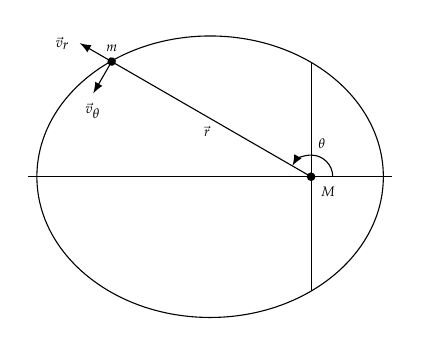
\begin{tikzpicture}[scale=.55]
      \def\a{4} % semi-major axis
      \def\b{3.25} % semi-minor axis
      \def\angle{150} % angle
      \draw ellipse ({\a} and {\b});% Draw the ellipse
      \draw ({sqrt(\a*\a-\b*\b)},-2.65)--({sqrt(\a*\a-\b*\b)},2.65);
      \draw (-\a-.2,0)--(\a+.2,0);
      \fill ({sqrt(\a*\a-\b*\b)},0) circle(.1) node[below right]{\tiny $M$};
      \begin{scope}[rotate around={\angle:({sqrt(\a*\a-\b*\b)},0)}]
        \draw[->]({sqrt(\a*\a-\b*\b)},0)--(8.5,0)
        node[pos=.45,below]{\tiny$\vec r$}
        node[left]{\tiny $\vec v_r$};
        \draw[->](7.65,0)--(7.65,.85) node[below]{\tiny $\vec v_\theta$};
        \fill (7.65,0) circle(.1) node[above]{\tiny $m$};
      \end{scope}
      \draw[->]({sqrt(\a*\a-\b*\b)+.5},0) arc(0:\angle:.5)
      node[pos=.4,above]{\tiny$\theta$};
%      \draw[<->]({sqrt(\a*\a-\b*\b)-.2},0)--({sqrt(\a*\a-\b*\b)-.2},-2.65)
%      node[midway,left]{\tiny$r_0$};
    \end{tikzpicture}
    
    \column{.7\textwidth}
    \begin{itemize}
    \item $\vec v_\theta$ means a centripetal acceleration toward $M$
    \item Changes in $\vec v_r$ (i.e.\ accceleration in the radial direction)
      also means a force along $\hat r$
    \item Both components of acceleration are due entirely to gravitational
      force toward $M$
    \item Applying second law of motion gives a complicated (at least for
      students new to the concept) ordinary differential equation.
    \end{itemize}
  \end{columns}
  \vspace{.1in}A full description for solving the differential equation is
  presented in the accompanied handout for anyone interested.
\end{frame}



\begin{frame}{Kepler's First Law: Law of Ellipses}
  The solution to the ODE is the expression for $r(\theta)$, with eccentricity
  $e$ determined by a constant $B$ based on initial condition (how the planet
  is formed):

  \eq{-.1in}{
    r=\left[\frac{L^2}{GMm^2}\right]\frac1{1+e\cos\theta}
    \quad\text{where}\quad  e=\frac{BL^2}{GMm^2}
  }

  The semi-major axis is the average value between the minimum and maximum
  values of $r$:
  
  \eq{-.1in}{
    a=\frac12(r_\text{min} + r_\text{max})
    =\left[\frac{L^2}{GMm^2}\right]\frac1{1-e^2}
  }

  We can rearrange the terms to see that this is the equation for an ellipse.
\end{frame}



\subsection{Third Law}

\begin{frame}{Kepler's Third Law: The Law of Periods}
  \centering
  \fbox{
    \begin{minipage}{.97\textwidth}
      \textbf{Law of Periods: The square of the orbital period of a planet
        is proportional to the cube of the semi-major axis of its orbit.}
    \end{minipage}
  }

  \vspace{.2in}\pic{.45}{kep8}
\end{frame}



\begin{frame}{Kepler's Third Law: The Law of Periods}
  The area swept by the planet through one orbital period is the areal velocity
  (constant!) integrated by time, from $t=0$ to $t=T$:

  \eq{-.1in}{
    A=\int\dl A=\int_0^T\diff At\dl t=\frac L{2m}\int_0^T\dl t=\frac L{2m}T
  }
  
  But this area is an ellipse, given by the equation based on $a$ (semi-major
  axis), $b=a\sqrt{1-e^2}$ (semi-minor axis):

  \eq{-.1in}{
    A=\pi ab=\pi a^2\sqrt{1-e^2}
  }

  Equating two equations above and squaring both sides give this expression:

  \eq{-.1in}{
    T^2=\frac{m^2}{L^2}4\pi^2a^4(1-e^2)
  }
\end{frame}



\begin{frame}{Kepler's Third Law: The Law of Periods}
  But we also (from proving the first law) have:

  \eq{-.1in}{
    a(1-e^2)=\frac{L^2}{GMm^2}
  }

  Substituting this expression into the equation for the period, and after
  some simple algebra, we end up with this expression:

  \eq{-.1in}{
    \boxed{T^2=\left[\frac{4\pi^2}{GM}\right] a^3}
  }
\end{frame}


%\begin{frame}{Orbital Speed}
%  \eq{.0in}{
%    \boxed{v_\mathrm{orbit}=\sqrt{\frac{GM} r}}
%  }
%  Assumptions:
%  \begin{itemize}
%  \item The orbit of the $m$ must be perfectly circular
%  \item That $M\gg m$, and $M$ can therefore be treated as a fixed point
%  \end{itemize}
%  Reality:
%  \begin{itemize}
%  \item As $m$ is subjected to a centripetal force supplied by the gravity from
%    $M$,\\
%    $M$ is also subjected to a centripetal force supplied by the gravity from
%    $m$.
%  \item $m$ does not actually orbit about the center of $M$, but rather, the
%    center of mass between $M$ and $m$.
%  \end{itemize}
%\end{frame}



\subsection{Clarifications}

\begin{frame}{Reality of Orbital Motion}
  As always, nothing is as simple as is first seems
  \begin{itemize}
  \item Most AP Problems will be circular instead of elliptical, but you must
    know the nature of gravitational force (conservative, central)
  \item The analysis on the slides shown assumes a small mass $m$ orbiting
    around a large mass $M$. In reality:
    \begin{itemize}
    \item Just as planets experience a gravitational force by the Sun, the Sun
      experiences a gravitational force from the planets
    \item The smaller mass $m$ does not actually orbit about the center of $M$,
      but rather, the \emph{center of mass between $M$ and $m$}
    \item Especially important when the two objects orbiting each other has
      similar masses (e.g.\ a binary star system)
    \end{itemize}
  \end{itemize}
\end{frame}




%\begin{frame}{Reduced Mass}
%  When two objects are orbiting each other, the center of mass of the system is
%  along the line between them:
%  \begin{center}
%    \begin{tikzpicture}
%      \begin{scope}[rotate=23]
%        \draw[very thick,->](0,0)--(3,0) node[midway,below]{$\vec r_1$};
%        \draw[very thick,->](0,0)--(-1.8,0) node[midway,above]{$\vec r_2$};
%        \fill (3.1,0) circle(.1) node[right]{$m_1$};
%        \fill (-1.9,0) circle(.1) node[left]{$m_2$};
%        \fill[red!80!black] (0,0) circle(.1) node[below]{$M$};
%      \end{scope}
%    \end{tikzpicture}
%  \end{center}
%
%  \vspace{-.1in}The vectors $\vec r_1$ and $\vec r_2$ are relative to the
%  center of mass, and the relative position $\vec r$ velocity $\vec{v}$ and
%  acceleration $\vec{a}$ between $m_1$ and $m_2$ are therefore:
%  
%  \eq{-.2in}{
%    \vec r=\vec r_2 - \vec r_1\quad
%    \vec{v}=\vec{v}_2 - \vec{v}_1\quad
%    \vec{a}=\vec{a}_2 - \vec{a}_1
%  }
%\end{frame}
%
%
%
%\begin{frame}{Reduced Mass}  
%  From Newton's third law, we know that the gravitational force exerted by
%  $m_1$ on $m_2$ is opposite the force exerted by $m_2$ on $m_1$:
%
%  \eq{-.2in}{
%    m_1\vec{a}_1+m_2\vec{a}_2=0
%  }
%
%  \vspace{-.2in}Substituting the expression for relative acceleration, we have:
%
%  \eq{-.2in}{
%    \vec{a}=\vec F_g\left[\frac{1}{m_1}+\frac{1}{m_2}\right]=
%    \vec F_g\left[\frac{m_1+m_2}{m_1m_2}\right]=\frac{\vec F_g}{\mu}
%  }
%  
%  We can now define a new concept called \textbf{reduced mass}:
%  
%  \eq{-.2in}{
%    \mu=\frac{m_1m_2}{m_1+m_2}
%  }
%\end{frame}
%
%\begin{frame}{An Equivalent System}
%  The orbit of one of the masses in a binary system is equivalent to the motion
%  of the reduced mass orbiting around a point at relative distance $r$ where
%  the total mass $M$ is placed. The magnitude of $r$ is the same as the
%  relative distance $r$ in the development on previous slides.
%  \vspace{-.2in}\begin{center}
%    \begin{tikzpicture}
%      \begin{scope}[rotate=23]
%        \draw[very thick,->](0,0)--(4.8,0) node[midway,below]{$\vec r$};
%        \draw[very thick,->,red!70!black](4.87,0)--(4.5,1)
%        node[above]{$\vec{v}$};
%        \fill[red!70!black] (0,0) circle(.15) node[below]{$M$};
%        \fill (4.87,0) circle(.07) node[right]{$\mu$};
%      \end{scope}
%    \end{tikzpicture}
%  \end{center}
%\end{frame}


\begin{frame}{Binary System}
  \begin{columns}
    \column{.45\textwidth}
    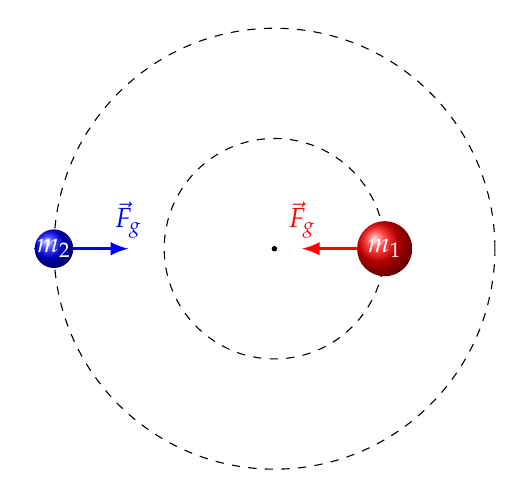
\begin{tikzpicture}[scale=.35]
      \fill circle(.1);
      \draw[dashed] circle(4);
      \draw[dashed] circle(8);
      \shade[ball color=red] ( 4,0) circle(1)  node[white]{$m_1$};
      \shade[ball color=blue](-8,0) circle(.7) node[white]{$m_2$};
      \draw[very thick,->,blue](-7.3,0)--(-5.3,0) node[above]{$\vec F_g$};
      \draw[very thick,->,red](3,0)--(1,0) node[above]{$\vec F_g$};
    \end{tikzpicture}

    \column{.55\textwidth}
    In a binary star system, two stars orbit around their center of mass. Both
    have the same period, and the gravitational force provides the centripetal
    force, but this time, the distance to the center of motion is empty space.
  \end{columns}
\end{frame}
\end{document}
